\documentclass[a4paper,11pt,fleqn]{article}

\usepackage[utf8]{inputenc}
%\usepackage[swedish]{babel}
\usepackage[lighttt]{lmodern}

%\usepackage{amsmath}
%\usepackage{amssymb}
%\usepackage{amsthm}
%\usepackage{listings}
%\usepackage{parskip}
%\usepackage{enumerate}
%\usepackage{tikz}
\usepackage{graphicx}


%\usepackage{geometry}
%\geometry{
%	%top=1.5in,
%	bottom=1.5in
%}

\author{Andreas Hagesjö \and Daniel Pettersson \and
Magnus Hagmar \and Niclas Ogeryd \and Robert Nyquist}

\title{Modell över Sverige primärenergitillförsel \\ Kurs ENM155} 


\begin{document}
\pagenumbering{gobble} 
\maketitle
\newpage
\pagenumbering{arabic} 

\section{Introduktion}
Denna rapport innehåller en enkel modell utav Sveriges energisystem som det ser ut idag.
Den innehåller en matematisk modell samt en uppskattning utav Sveriges totala primärenergitillförsel.


\section{Metod}
Modellen är nerbruten i tre delar, industri, transport och bostäder som är de olika sektorerna.
För varje sektor så listas alla primärenergier som birdrar till respektive sektor. Varje primärenergi går sedan vidare till de olika sekundärenergierna som den bidrar till. Varje sekundär energi går till sist vidare till sektorn, alternativ till en ny sekundärenergi som i sin tur går vidare till en sektor eller ytterligare en sekundärenergi.
I Appendix B finns de matematiska formlerna för att räkna ut primarenergierna för varje enskild sektor.


\begin{itemize}
\item Då vi har brutit ner modellen i sektorer så följer de inte diagrammet i Figur 1 i lab PM.
Istället så ger flödesschemat i Appendix A en direkt bild utav våran implementation.


\item Modellen är byggd så att det går att ta reda på tillförseln av varje enskild primärenergi samt vilka typer av primärenergi, och mängedn, varje enskild sektor använder.
Det går även att räkna ut värden sekundärenerg för varje sektor med hjälp av modellen.

\item

Beskriv kortfattat hur man skulle gå till väga för att lägga till ett
nytt primärenergislag i er modell (till exempel solenergi). Samma sak för
ett nytt sekundärenergislag (till exempel vätgas genom elektrolys och
reformering).
\end{itemize}

\section{Resultat}
Presentera Sveriges totala primärenergitillförsel, samt uppdelat på
respektive energikälla.

\appendix
\section{Flödesschema}
\begin{figure}[h!]
	\centering 
 		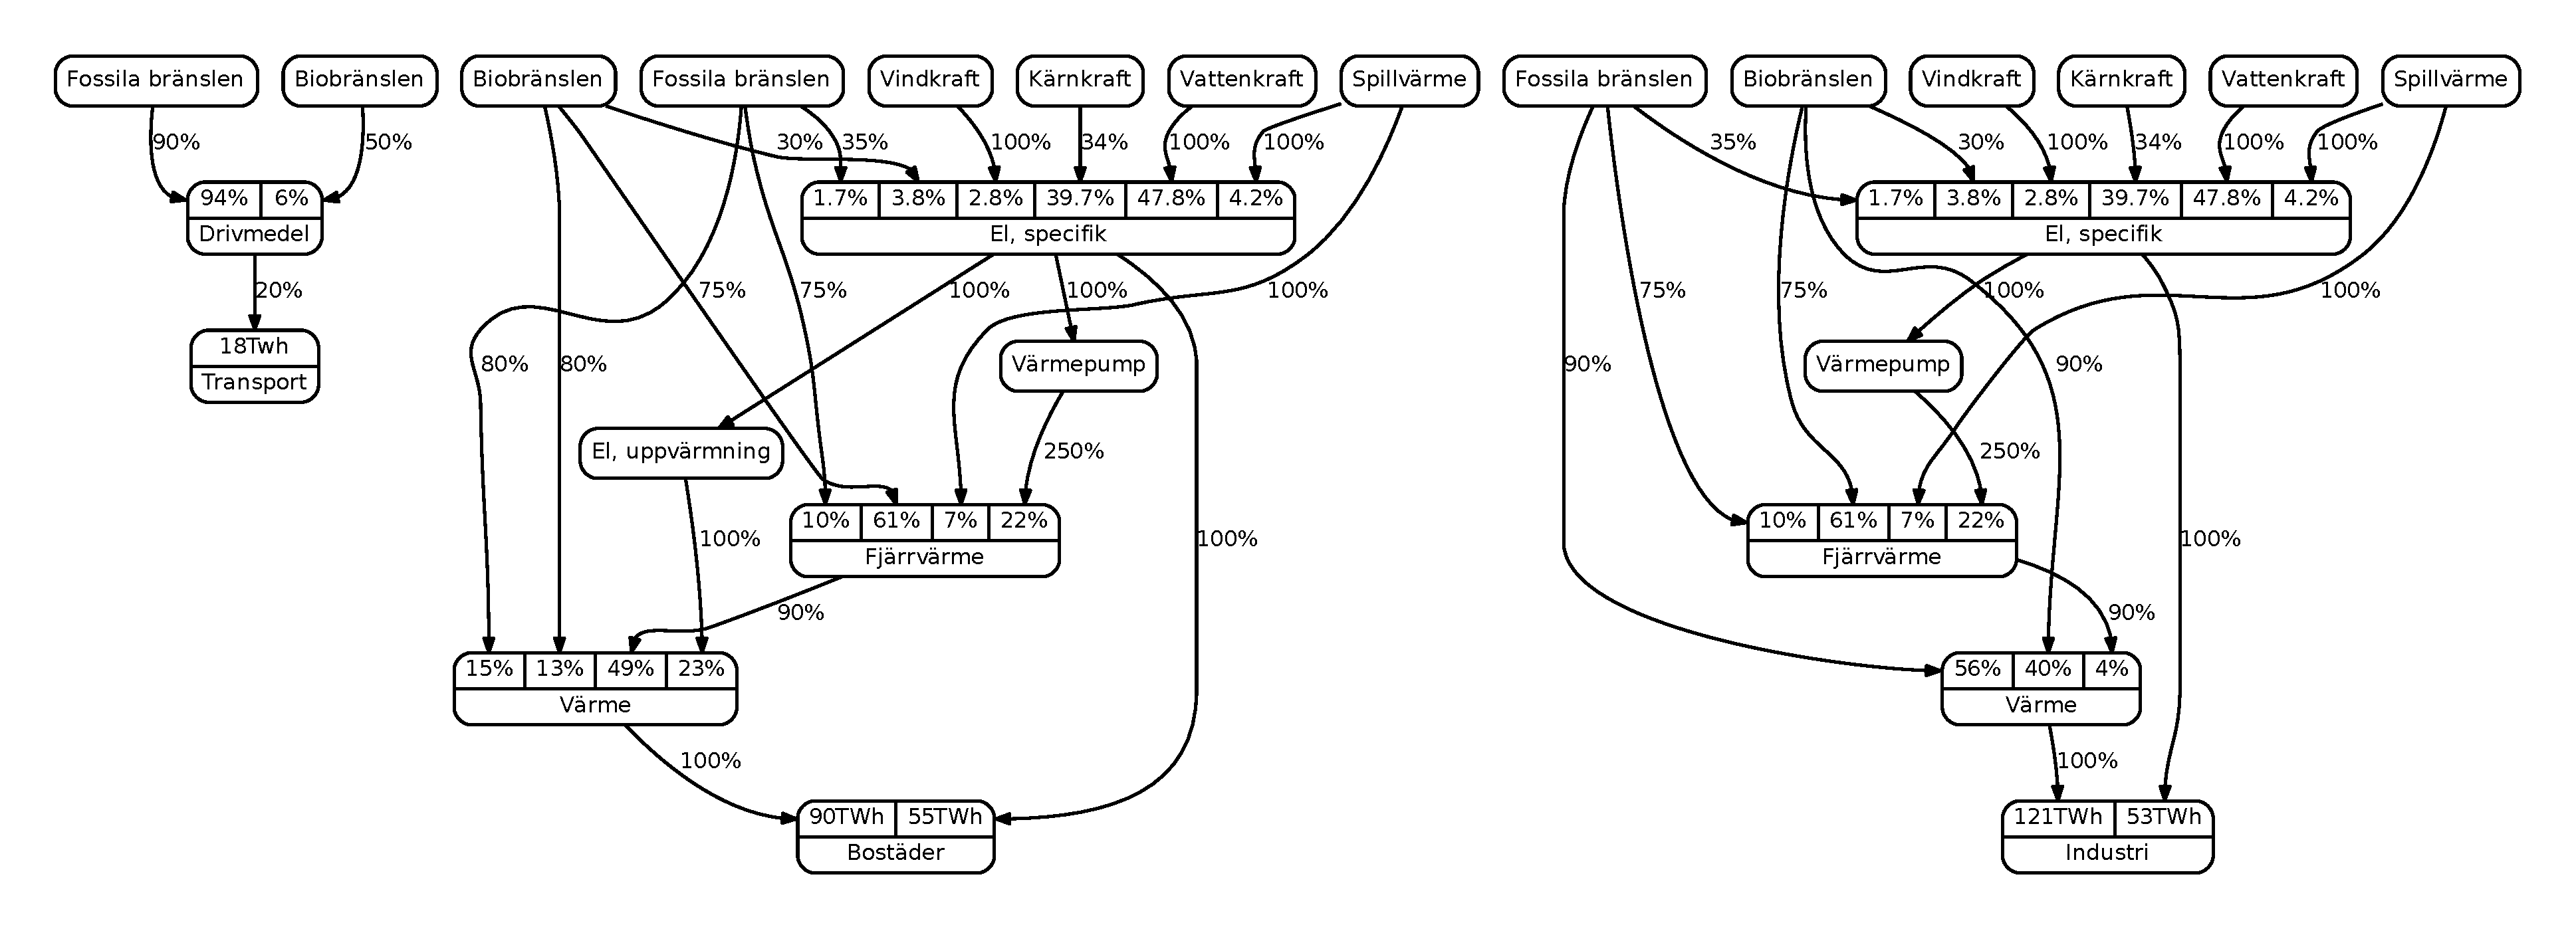
\includegraphics[scale = 0.2]{diagram.pdf}
		\label{diagram}
\end{figure}
\section {Matematisk modell}
\subsection{Transport}
\begin{figure}[h!]
	\centering 
 		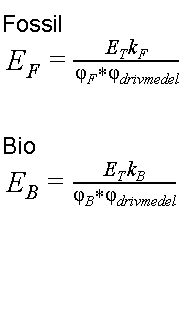
\includegraphics[scale = 0.75]{transport2.pdf}
		\label{diagram}
\end{figure}
\subsection{Bostäder}
\begin{figure}[h!]
	\centering 
 		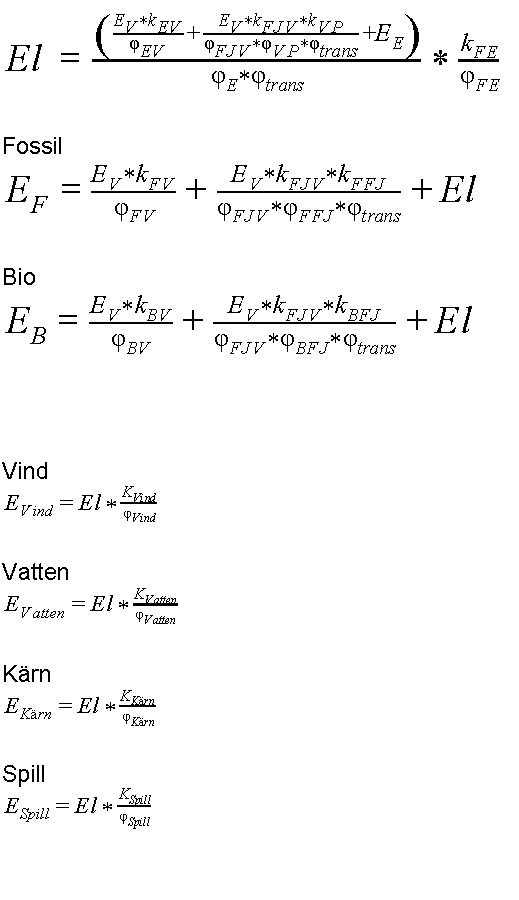
\includegraphics[scale = 0.75]{homes2.pdf}
		\label{diagram}
\end{figure}
\subsection{Industri}
\begin{figure}[h!]
	\centering 
 		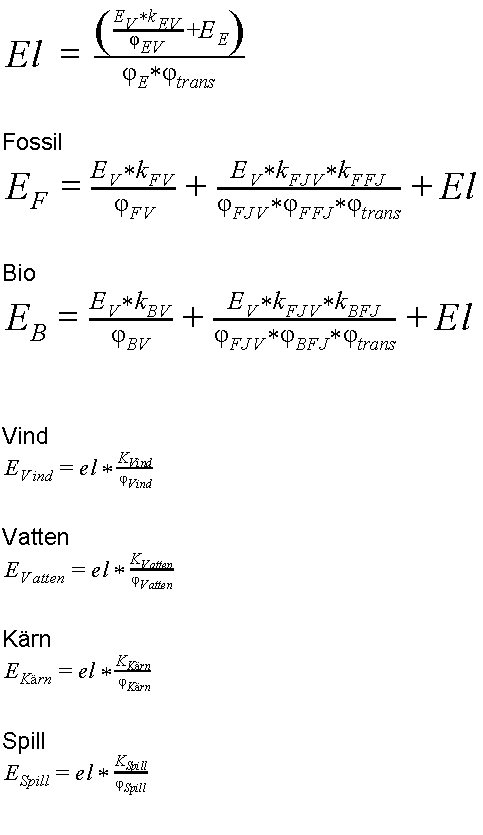
\includegraphics[scale = 0.75]{industri2.pdf}
		\label{diagram}
\end{figure}
\section{Programkod}
Bifoga koden

\end{document}

